\documentclass[]{article}
\usepackage{lmodern}
\usepackage{amssymb,amsmath}
\usepackage{ifxetex,ifluatex}
\usepackage{fixltx2e} % provides \textsubscript
\ifnum 0\ifxetex 1\fi\ifluatex 1\fi=0 % if pdftex
  \usepackage[T1]{fontenc}
  \usepackage[utf8]{inputenc}
\else % if luatex or xelatex
  \ifxetex
    \usepackage{mathspec}
  \else
    \usepackage{fontspec}
  \fi
  \defaultfontfeatures{Ligatures=TeX,Scale=MatchLowercase}
  \newcommand{\euro}{€}
\fi
% use upquote if available, for straight quotes in verbatim environments
\IfFileExists{upquote.sty}{\usepackage{upquote}}{}
% use microtype if available
\IfFileExists{microtype.sty}{%
\usepackage{microtype}
\UseMicrotypeSet[protrusion]{basicmath} % disable protrusion for tt fonts
}{}
\usepackage[margin=1in]{geometry}
\usepackage{hyperref}
\PassOptionsToPackage{usenames,dvipsnames}{color} % color is loaded by hyperref
\hypersetup{unicode=true,
            pdftitle={GVPT392(849): Intro to GIS for Social Science Research},
            pdfauthor={Nicholas Thompson},
            pdfsubject={Mid-Term Exam (extension granted)},
            pdfborder={0 0 0},
            breaklinks=true}
\urlstyle{same}  % don't use monospace font for urls
\usepackage{color}
\usepackage{fancyvrb}
\newcommand{\VerbBar}{|}
\newcommand{\VERB}{\Verb[commandchars=\\\{\}]}
\DefineVerbatimEnvironment{Highlighting}{Verbatim}{commandchars=\\\{\}}
% Add ',fontsize=\small' for more characters per line
\usepackage{framed}
\definecolor{shadecolor}{RGB}{248,248,248}
\newenvironment{Shaded}{\begin{snugshade}}{\end{snugshade}}
\newcommand{\KeywordTok}[1]{\textcolor[rgb]{0.13,0.29,0.53}{\textbf{{#1}}}}
\newcommand{\DataTypeTok}[1]{\textcolor[rgb]{0.13,0.29,0.53}{{#1}}}
\newcommand{\DecValTok}[1]{\textcolor[rgb]{0.00,0.00,0.81}{{#1}}}
\newcommand{\BaseNTok}[1]{\textcolor[rgb]{0.00,0.00,0.81}{{#1}}}
\newcommand{\FloatTok}[1]{\textcolor[rgb]{0.00,0.00,0.81}{{#1}}}
\newcommand{\ConstantTok}[1]{\textcolor[rgb]{0.00,0.00,0.00}{{#1}}}
\newcommand{\CharTok}[1]{\textcolor[rgb]{0.31,0.60,0.02}{{#1}}}
\newcommand{\SpecialCharTok}[1]{\textcolor[rgb]{0.00,0.00,0.00}{{#1}}}
\newcommand{\StringTok}[1]{\textcolor[rgb]{0.31,0.60,0.02}{{#1}}}
\newcommand{\VerbatimStringTok}[1]{\textcolor[rgb]{0.31,0.60,0.02}{{#1}}}
\newcommand{\SpecialStringTok}[1]{\textcolor[rgb]{0.31,0.60,0.02}{{#1}}}
\newcommand{\ImportTok}[1]{{#1}}
\newcommand{\CommentTok}[1]{\textcolor[rgb]{0.56,0.35,0.01}{\textit{{#1}}}}
\newcommand{\DocumentationTok}[1]{\textcolor[rgb]{0.56,0.35,0.01}{\textbf{\textit{{#1}}}}}
\newcommand{\AnnotationTok}[1]{\textcolor[rgb]{0.56,0.35,0.01}{\textbf{\textit{{#1}}}}}
\newcommand{\CommentVarTok}[1]{\textcolor[rgb]{0.56,0.35,0.01}{\textbf{\textit{{#1}}}}}
\newcommand{\OtherTok}[1]{\textcolor[rgb]{0.56,0.35,0.01}{{#1}}}
\newcommand{\FunctionTok}[1]{\textcolor[rgb]{0.00,0.00,0.00}{{#1}}}
\newcommand{\VariableTok}[1]{\textcolor[rgb]{0.00,0.00,0.00}{{#1}}}
\newcommand{\ControlFlowTok}[1]{\textcolor[rgb]{0.13,0.29,0.53}{\textbf{{#1}}}}
\newcommand{\OperatorTok}[1]{\textcolor[rgb]{0.81,0.36,0.00}{\textbf{{#1}}}}
\newcommand{\BuiltInTok}[1]{{#1}}
\newcommand{\ExtensionTok}[1]{{#1}}
\newcommand{\PreprocessorTok}[1]{\textcolor[rgb]{0.56,0.35,0.01}{\textit{{#1}}}}
\newcommand{\AttributeTok}[1]{\textcolor[rgb]{0.77,0.63,0.00}{{#1}}}
\newcommand{\RegionMarkerTok}[1]{{#1}}
\newcommand{\InformationTok}[1]{\textcolor[rgb]{0.56,0.35,0.01}{\textbf{\textit{{#1}}}}}
\newcommand{\WarningTok}[1]{\textcolor[rgb]{0.56,0.35,0.01}{\textbf{\textit{{#1}}}}}
\newcommand{\AlertTok}[1]{\textcolor[rgb]{0.94,0.16,0.16}{{#1}}}
\newcommand{\ErrorTok}[1]{\textcolor[rgb]{0.64,0.00,0.00}{\textbf{{#1}}}}
\newcommand{\NormalTok}[1]{{#1}}
\usepackage{graphicx,grffile}
\makeatletter
\def\maxwidth{\ifdim\Gin@nat@width>\linewidth\linewidth\else\Gin@nat@width\fi}
\def\maxheight{\ifdim\Gin@nat@height>\textheight\textheight\else\Gin@nat@height\fi}
\makeatother
% Scale images if necessary, so that they will not overflow the page
% margins by default, and it is still possible to overwrite the defaults
% using explicit options in \includegraphics[width, height, ...]{}
\setkeys{Gin}{width=\maxwidth,height=\maxheight,keepaspectratio}
\setlength{\parindent}{0pt}
\setlength{\parskip}{6pt plus 2pt minus 1pt}
\setlength{\emergencystretch}{3em}  % prevent overfull lines
\providecommand{\tightlist}{%
  \setlength{\itemsep}{0pt}\setlength{\parskip}{0pt}}
\setcounter{secnumdepth}{0}

%%% Use protect on footnotes to avoid problems with footnotes in titles
\let\rmarkdownfootnote\footnote%
\def\footnote{\protect\rmarkdownfootnote}

%%% Change title format to be more compact
\usepackage{titling}

% Create subtitle command for use in maketitle
\newcommand{\subtitle}[1]{
  \posttitle{
    \begin{center}\large#1\end{center}
    }
}

\setlength{\droptitle}{-2em}
  \title{GVPT392(849): Intro to GIS for Social Science Research}
  \pretitle{\vspace{\droptitle}\centering\huge}
  \posttitle{\par}
\subtitle{Mid-Term Exam (extension granted)}
  \author{Nicholas Thompson}
  \preauthor{\centering\large\emph}
  \postauthor{\par}
  \predate{\centering\large\emph}
  \postdate{\par}
  \date{9am Oct3 - 5pm Oct 9, 2016}


% Redefines (sub)paragraphs to behave more like sections
\ifx\paragraph\undefined\else
\let\oldparagraph\paragraph
\renewcommand{\paragraph}[1]{\oldparagraph{#1}\mbox{}}
\fi
\ifx\subparagraph\undefined\else
\let\oldsubparagraph\subparagraph
\renewcommand{\subparagraph}[1]{\oldsubparagraph{#1}\mbox{}}
\fi


\begin{document}
\maketitle

The following coverages can be found in the PACD8 folder.

\begin{enumerate}
\def\labelenumi{\arabic{enumi}.}
\item
  PA\_CD8\_Voterfile \(=\) all registered voters for Pennsylvania,
  Congressional District 8. This is north-suburban Philadelphia,
  including all of Bucks and part of Montgomery Counties.
\item
  PA\_CD8\_Boundary \(=\) the outline for CD 8.
\item
  PA\_and\_NJ\_Counties \(=\) County boundaries for the two states.
\item
  Four States = State boundaries for PA, DE, NJ, and MD.
\item
  CD8\_PA\_Pct\_Data\_2012 \(=\) voter precinct data for 2012.
\item
  Mont\_County\_Recent\_Movers\_10\_12.
\item
  Bucks\_County\_Recent\_Movers\_10\_12.
\item
  CD8\_Places.
\item
  PA CD8\_Tracts.
\end{enumerate}

Three files above contain points for voters at their residences. These
are 1, 6, and 7. For these files, the following columns contain
important information:

Age (and Year Born) \(=\) the age of the voter in 2012.

Rep\_Party, Dem\_Party, Ind\_Unaf\_Party \(=\) the party registration of
the voter: Rep \(=\) Republican, Dem \(=\) Democratic, and Ind\_Unaf
\(=\) Independent/Unaffiliated.

And there are other items that will be less important for this exercise.

\begin{center}\rule{0.5\linewidth}{\linethickness}\end{center}

For the following questions, use whatever tools you deem appropriate
form the ArcGIS package, but be sure to describe what you did to address
the questions. Be resourceful, but you need not write more than one page
in response to each question.

\clearpage

1. Aggregate the voter and mover data to the census tract level for PA
CD8.

~~~~~~To aggregate the data, I used a three phase process with multiple
steps in each phase. In Phase 1, I imported the data using the catalogue
in ArcMap. To import the data I first created a geodatabase file named
\texttt{exam}. Here I imported all exam shapefiled included in the
provided exam folder by right clicking on the \texttt{exam.gdb} and
selecting import from multiple. Next I systemtaically added four file
layers to the ArcMap table of contents:

~~~~~~a. PA\_CD8\_Voterfile (hereafter depicted as \texttt{voter});

~~~~~~b. Mont\_County\_Recent\_Movers\_10\_12 (hereafter depicted as
\texttt{MC});

~~~~~~c. Buck\_County\_Recent\_Movers\_10\_12 (hereafter depicted as
\texttt{BC});

~~~~~~d. PA\_CD8\_Tracts (hereafter depicted as \texttt{tracts}).

This was the end of Phase 1.

~~~~~~In Phase 2, I reviewed the data and deleted unnecessary fields.
The number is too great to depict which were removed. I kept essential
fields outlined in the instructions above, as well as some others that I
anticipated would be necessary (including \texttt{MOVER} from the
\texttt{voter} file, \texttt{ozipcode} and \texttt{dzipcode} from
\texttt{MC} and \texttt{BC}, and \texttt{ORNIC}, \texttt{DRNIC}, and
\texttt{RNIC} from \texttt{voter}, \texttt{BC}, and \texttt{MC}). The
combination of fields chosen allowed me to manipulate the data to
achieve the desired results. I removed fields by double-clicking on each
layer in the table of contents and navigating to the \texttt{Fields}
tab. After clearing all of the fields, I was able to check only the
fields I wanted to keep. Next, I exported the data into new layers
within the geodatabase. This data management process ended Phase 2.

~~~~~~In Phase 3, I used the \texttt{Spatial\ Join} feature (hereafter
known as \texttt{SJ}) to systemtaically join the layers. First I
conducted a \texttt{SJ} of \texttt{voters} to \texttt{tracts} and
created a new layer called \texttt{tracts01}. Next I created the
following \texttt{SJ}s:

~~~~~~a. \texttt{tracts} \(+\) \texttt{BC} \(=\) \texttt{tracts02}

~~~~~~b. \texttt{tracts} \(+\) \texttt{MC} \(=\) \texttt{tracts04}

~~~~~~c. \texttt{tracts01} \(+\) \texttt{tracts02} \(=\)
\texttt{tracts03}

~~~~~~d. \texttt{tracts03} \(+\) \texttt{tracts04} \(=\)
\texttt{tracts07}

The last combination created a spatially joined dataset depicting the
north-suburban part of Philadelphia.

\begin{itemize}
\tightlist
\item
  Then compute and calculate the Democratic \(\%\) of total registered
  voters (10 points).
\end{itemize}

To compute and calculate the Democratic \(\%\) of total registered
voters I needed to create a new field in the \texttt{BC} and \texttt{MC}
shapefiles. I completed these computations prior to merging all of the
data to ensure that they were carried over in each of the \texttt{SJ}s.
First, I created a new field called \texttt{vote\_total}. Using the
field calculator tool, I added the \texttt{Republican},
\texttt{Democratic}, and \texttt{Independent} fields together. This
produced a one in each row of the \texttt{vote\_total}. Next, I used the
statistics tool to calculate the total sum of from the
\texttt{Democratic} field and the the sum from the \texttt{vote\_total}
fields. I conducted statistical analysis before and after conducting the
joins. The Table 1 below shows the outcomes. Note there is no
significant difference in the percentages either pre- or post-join.

\begin{table}[]
\centering
\caption{Percentage of Democratic Voters}
\begin{tabular}{ccc}
Field       & Pre-Join & Post-Join \\
\hline
Democratic  & 71,048   & 133,467   \\
vote\_total & 540,451  & 1,019,887 \\
\hline
\hline
Percentages & 53.23 \% & 52.99 \% 
\end{tabular}
\end{table}

\begin{itemize}
\tightlist
\item
  Compute and calculate the Democratic \(\%\) of total movers in Bucks
  and Montgomery counties (10 points).
\end{itemize}

To calculate the percentage of democratic movers I created two fields in
\texttt{BC} and \texttt{MC} once callde \texttt{zip\_dif} and another
called \texttt{move2}. The \texttt{zip\_dif} field captured a difference
between the originating zip code (\texttt{ozipcode}) of each voter in
the respective counties and the destination zip code
(\texttt{dzipcode}). Next, a phython code converted the
\texttt{zip\_dif} field into a \(1\) or a \(0\). This allowed me to
total the number of people that moved from one zip code to another.
Table 2 shows the results of this computation.

\begin{Shaded}
\begin{Highlighting}[]
\NormalTok{def }\KeywordTok{is_positive}\NormalTok{(x):}
\StringTok{  }\NormalTok{if (}\KeywordTok{abs}\NormalTok{(x)>}\DecValTok{0}\NormalTok{):}
\StringTok{    }\NormalTok{return }\DecValTok{1}
  \KeywordTok{elif} \NormalTok{(}\KeywordTok{abs}\NormalTok{(x)==}\DecValTok{0}\NormalTok{):}
\StringTok{    }\NormalTok{return }\DecValTok{0} 
\end{Highlighting}
\end{Shaded}

\begin{table}[]
\centering
\caption{Percentage of Democratic Movers}
\label{my-label}
\begin{tabular}{cccc}
Field       & Montgomery & Bucks    & Sum      \\
\hline
Democratic  & 2,016      & 22,555   & 24,571   \\
move\_total & 4,620      & 42,040   & 46,660   \\
\hline
\hline
Percentages & 43.63 \%   & 53.65 \% & 52.66 \%
\end{tabular}
\end{table}

\begin{itemize}
\tightlist
\item
  Produce two maps of these percentages.
\end{itemize}

To produce my maps I followed some formatting guidelines. First, I
always included a legend, scale, and north seeking arrow. Also included
was my name as the author and the date I finalized the map. For this
first set of maps I normalized the \texttt{Sum\_Sum\_Democratic}
variable over the \texttt{Sum\_Sum\_vote\_total} for the first map (as
labeled in Figure 1). I normalized the \texttt{Sum\_Sum\_Democratic}
variable over the \texttt{Sum\_Sum\_vote\_total} variable for the second
requirement.

This depicts a strong concentration of Democratic voters located in the
southeastern portion of the country. Democratic voters show a propensity
for migration with a large percentage moving in and around the
southeastern portion of the county.

Note that this data does not reflect the \texttt{MOVER} field from the
\texttt{MC} dataset. The \texttt{MOVER} variable was not used because it
was only available in the \texttt{MC} dataset and only depicted a small
swath of migration running from northwest to southeast along the
southwestern third of the county. All map figures will be available in
the Appendix.

2. How would you characterize the spatial distribution of Republicans,
Democrats, and Independents in PA CD8? Write up two paragraphs based on
what you have found, describing how you used ArcGIS to address the
question. (20 points)

Democrats, by and large, tend to be located in the south eastern part of
the map (which is northern Philadelphia). Republicans are a
significantly lesser amount of the population and tend to inhabit the
norther part of the voting district, with a concentration in the center
of Montgomery county in the southwest. Independents show similar
patterns to the Republicans but on a much smaller scale.

I used a percentage of total voters for each party and compared them to
one another, as depicted in Figure 2. This distribution by percentage
was calculated using the \texttt{Sum\_Sum\_Democrat},
\texttt{Sum\_Sum\_Republican} and \texttt{Sum\_Sum\_Independent}
variables normalized by \texttt{Sum\_Sum\_vote\_total} variable. I
utilized a five quantile break.

3. The data included also show two populations of recent movers from
inside PA and from nearby states. How do the recent movers in
Montogomery and Bucks counties compare by age and by party registration
to the entire PA\_CD8 voting populations? Explain your answer in no more
than one page.

To answer this question I pulled the descriptive statistics for each
dataset (\texttt{BC}, \texttt{MC}, \texttt{voter}) and collected the
number of people that voted in each party, the party means, and the
party standard deviations (Table 3). I also collected the mean, standard
deviation, minimum, and maximum values of the voters from each of the
three datasets (Table 4).

The Montgomery county movers are represented by a higher percentage of
Republicans than Democrats (Independents are behing Republicans and
Democrats in all three datasets. The Bucks county Democratic movers
(\(46.10\%\)) have a significantly higher percentage than Montgomery
county movers (\(37.68\%\)). This indicates that either Democrats in
Bucks county are migrating at higher rates, or that the percentage of
voters in both counties falls around those means.

One way to differentiate between the two possibilities is to compare the
means of the total voter population from the district. If we assume a
normal distribution of Republican, Democratic, and Independent voters
throughout the district then the averages of \(34.13\%\) for
Republicans, \(52.63\%\) for Democratic party voters, and \(12.10\%\)
for Independent voters should represent similar means the two counties.

The Republican numbers in Bucks county are close to the overall voter
mean, but the Montgomery mean is higher. This indicates that Republicans
are migrating to Montgomery county. The mean of Democratic voters in
both Bucks and Montgomery counties is significantly lower than in the
\texttt{voter} database. This may indicate less migration for Democratic
voters.

The age demographics do not tell us as much without a geographic
dispersion. The mean and standard deviation of the three data sets is
relatively similar, as depicted in Table 4. As depicted in Figures 3-5,
the age dispersion.

In order to complete the maps I combined a choropleth map of each party
(red for Repubulican, blue for Democrat, green for Independent) with a
centroid map of the overall voting population. This normalized the
regiserted voters by each age group. While the ages look identical in
each map, the scales of the circles are different. Note the low numbers
of 18-29 year old voters in comparison to 30-49 year olds.

To create the centroid maps I followed this sequence. First I created XY
coordinate for each dataset by adding a new X and Y field respectively.
Next using the ``Calculate Gemoetry'' function for each X and Y
respecitvely. Next, I joined the \texttt{tracts} map with the
\texttt{BC}, \texttt{MC}, and \texttt{voter} data sets. Then I exported
the joined tract datasets to a \texttt{tractCentroids} table. This table
now had the centroids for each voting block.

To finalize the method I created a feature class from the XY
\texttt{tractCentroids} table. Opening the cataloge in ArcMap, I right
clicked on \texttt{trackCentroids} and clicked ``Create Feature Class''
\textgreater{} ``From XY Table''. I make the coordinate system the same
as all of my other maps, the South Pennsylvania 1984. Finally, I saved
the file as a File and Personal Geodatabase called
\texttt{voterTractCentroids}.

\begin{table}[]
\centering
\caption{Descriptive Statistics by Party}
\label{my-label}
\begin{tabular}{ccccc}
Dataset    & Party       & Vote Totals & Mean   & Std\_Dev \\ \hline
Montgomery & Republican  & 2230         & 0.4167 & 0.4930    \\
Montgomery & Democratic  & 2016         & 0.3768 & 0.4845   \\
Montgomery & Independent & 1043         & 0.1949 & 0.3962   \\ \hline
Bucks      & Republican  & 16808        & 0.3436 & 0.4748   \\
Bucks      & Democratic  & 22555        & 0.461  & 0.4984   \\
Bucks      & Independent & 8979         & 0.1835 & 0.3871   \\ \hline
Voter      & Republican  & 46085        & 0.3413 & 0.4742   \\
Voter      & Democratic  & 71048        & 0.5263 & 0.4993   \\
Voter      & Independent & 16334        & 0.121  & 0.3261  \\ \hline \hline
\end{tabular}
\end{table}

\begin{table}[]
\centering
\caption{Descriptive Statistics by Age}
\label{my-label}
\begin{tabular}{lllll}
\multicolumn{1}{c}{Data Set} & \multicolumn{1}{c}{Mean} & \multicolumn{1}{c}{\begin{tabular}[c]{@{}c@{}}Standard \\ Deviation\end{tabular}} & \multicolumn{1}{c}{Min} & \multicolumn{1}{c}{Max} \\ \hline
Montgomery                   & 43.81                    & 16.73                                                                             & 20                      & 104                     \\
Bucks                        & 44.83                    & 15.99                                                                             & 20                      & 104                     \\
Voter Data                   & 49.57                    & 17.50                                                                             & 0                       & 112                    \\ 
\hline 
\hline
\end{tabular}
\end{table}

\clearpage

4. Are movers more likely to relocate to particular locations than the
general voter populations within PA CD8? Or are they geoographically
distributed about the same way? Explain what you find in no more than
one page.

Based upon the analysis form the maps generated in Figures 3-5, the
propensity for 18-29 year olds is to reside in large numbers in
Philadeliphia across the spectrum of voting preferences. People in the
30-49 age blocks are more likely to live in the more rural areas of
bucks county, with a strong showing in the more suburban areas (there
are a large numer in the city, but less than the younger voting block).
Finally, the oldest block of voters is more broadly dispersed and in
generally smaller numbers overall.

The migration pattern appears to be that younger people migrate to the
city, whil middle aged people have a propensity to migrate back to the
suburbs. Seniors are likely to live in all of the areas in a similar
pattern to middle aged voters.

\subparagraph{5. How many Bucks County voters live within one half-mile
of the border with Philadelphia? (10
points)}\label{how-many-bucks-county-voters-live-within-one-half-mile-of-the-border-with-philadelphia-10-points}

To answer questions \(5, 6,\) and \(7\) I used the following processes
and steps. Noted differences are discussed in each question, but
generally a process or step for questions 6 and 7 follow described
processes or steps described in the following discussion.

There are \(10,318\) voters in Bucks County within one half of a mile of
the border with Philadelphia. I found this information through the
following process:

\begin{enumerate}
\def\labelenumi{\alph{enumi}.}
\tightlist
\item
  Step 1: Identify data to use:
\end{enumerate}

\begin{itemize}
\tightlist
\item
  The \texttt{voters} dataset and the \texttt{PA\_and\_NJ\_counties}
  dataset. I used the attribute tables from each. A single entry in the
  \texttt{PA\_and\_NJ\_counties} dataset identifies the boundary of
  Philadelphia (object ID \#\(72\)). To find this quickly and select it
  I sorted ascending the \texttt{City\_Boundary} field and scrolled to
  the one indicating Philadelphia.
\end{itemize}

\begin{enumerate}
\def\labelenumi{\alph{enumi}.}
\setcounter{enumi}{1}
\tightlist
\item
  Step 2: I needed to isolate the Bucks county voters within the
  \texttt{voters} dataset. I opened the attribute table and identified
  the field I needed to use (\texttt{JURISNAME}). Selecting by
  attribute, from the selection menue, I chose the \texttt{voter} layer
  \textgreater{} Method: create new selection \textgreater{} double
  click \texttt{JURISNAME} \textgreater{} = \textgreater{} ``Get Unique
  Values'' \textgreater{} double click \texttt{Bucks\ County}
  \textgreater{} Apply \textgreater{} Ok.
\end{enumerate}

\begin{itemize}
\tightlist
\item
  Next I exported the selected features to a new
  \texttt{File\ and\ Personal\ Geodatabase\ Feature\ Class} called
  \texttt{Voter\_BucksCty} \textgreater{} Export Data \textgreater{}
  Selected Records \textgreater{} Output Table. Next I went to the
  catalog and put the new \texttt{Voter\_BucksCty} into the Table of
  Contents.
\end{itemize}

\begin{enumerate}
\def\labelenumi{\alph{enumi}.}
\setcounter{enumi}{1}
\tightlist
\item
  Step 3: To identify the voters within a half of a mile (\(0.5\)
  miles), I ``Select by Location'' from the ``Selection'' menu.
\end{enumerate}

\begin{itemize}
\tightlist
\item
  Select only \texttt{Voter\_BucksCty} layer in the ``Target Layers''
  dialogue box \textgreater{} Selection method: ``Select from Features''
  \textgreater{} Source layer: \texttt{PA\_and\_NJ\_counties} (with
  Philadelphia selected as noted above) \textgreater{} Spatial selection
  method for target features: ``are within a distance of the source
  layer feature'' \textgreater{} distance = \(0.5\) \textgreater{} unit
  of measure: ``miles''.
\end{itemize}

\begin{enumerate}
\def\labelenumi{\alph{enumi}.}
\setcounter{enumi}{2}
\tightlist
\item
  Step 4: Open the \texttt{Voter\_BucksCty} attribute table and ``show
  selected records''. At the bottom there are two numbers: \(10,318\)
  records selected of \(425,956\) total records.
\end{enumerate}

\begin{enumerate}
\def\labelenumi{\arabic{enumi}.}
\setcounter{enumi}{5}
\tightlist
\item
  How many Bucks County voters live within one mile of the border with
  Philadelphia? (10 points)
\end{enumerate}

There are \(17,206\) voters in Bucks County within one mile of
Philadelphia.

To answer this question I already had the base processes and layers
compiled. To change the distance I returned to ``Selection''
\textgreater{} ``Select by Location''. I kept all of the information the
same, but I changed the distance from \(0.5\) miles to (\(1.0\)) miles.
Next, I returned to the \texttt{Voter\_BucksCty} attribute table and
recorded the new calculated numbers: \(17,206\) records selected of
\(425,956\) total records.

\begin{enumerate}
\def\labelenumi{\arabic{enumi}.}
\setcounter{enumi}{6}
\tightlist
\item
  What percentage are those two figures of the total Bucks County voter
  population?
\end{enumerate}

To answer this question I have all of the data I need from the previous
questions. Arithmatic reveals the answer:

\begin{itemize}
\item
  Voters residing within \(\frac{1}{2}\) mile:
  \(\frac{10,318}{425,956} = 0.0242\), or \(2.42\%\)
\item
  Voters residing within \(1\) mile:
  \(\frac{17,206}{425,956} = 0.0404\), or \(4.04\%\)
\end{itemize}

\section{Appendix}\label{appendix}

\begin{figure}[htbp]
\centering
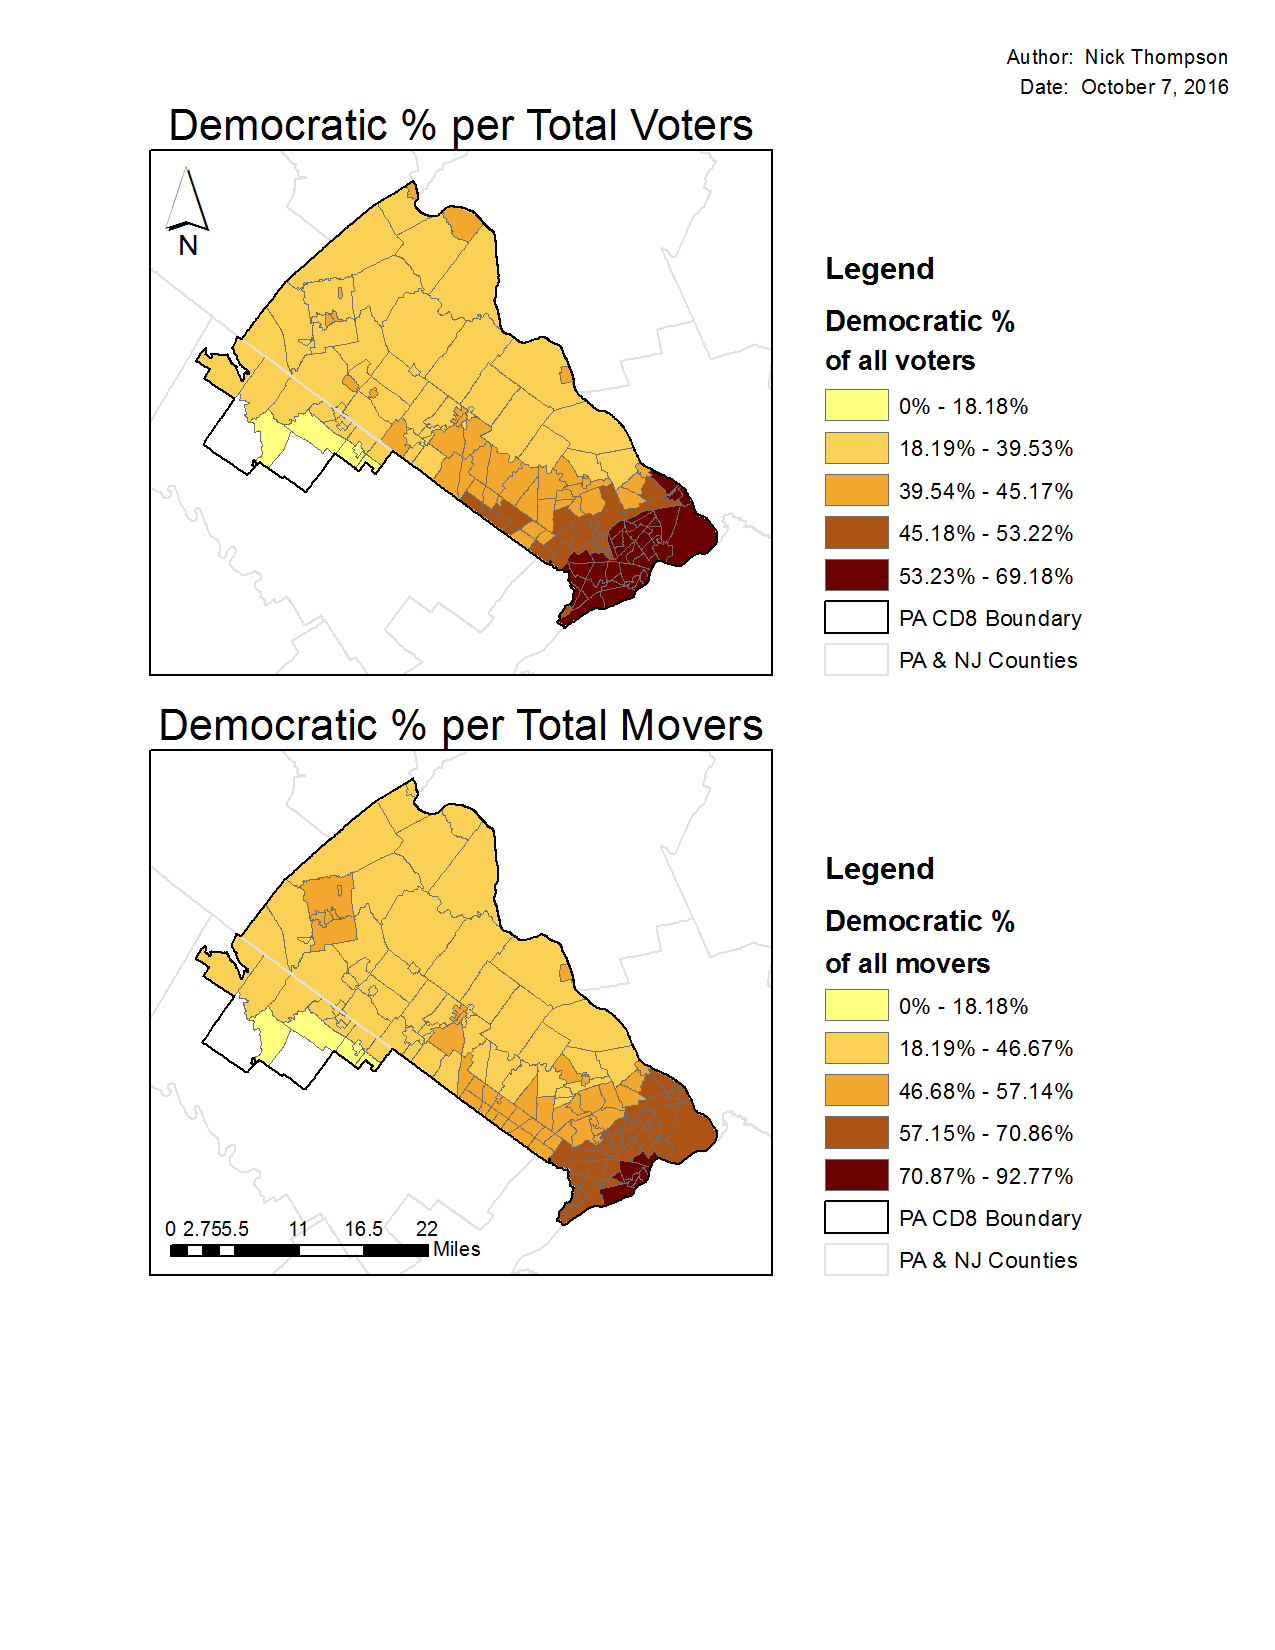
\includegraphics{question_1-2.png}
\caption{Figure 1: Democratic Voters and Movers}
\end{figure}

\begin{figure}[htbp]
\centering
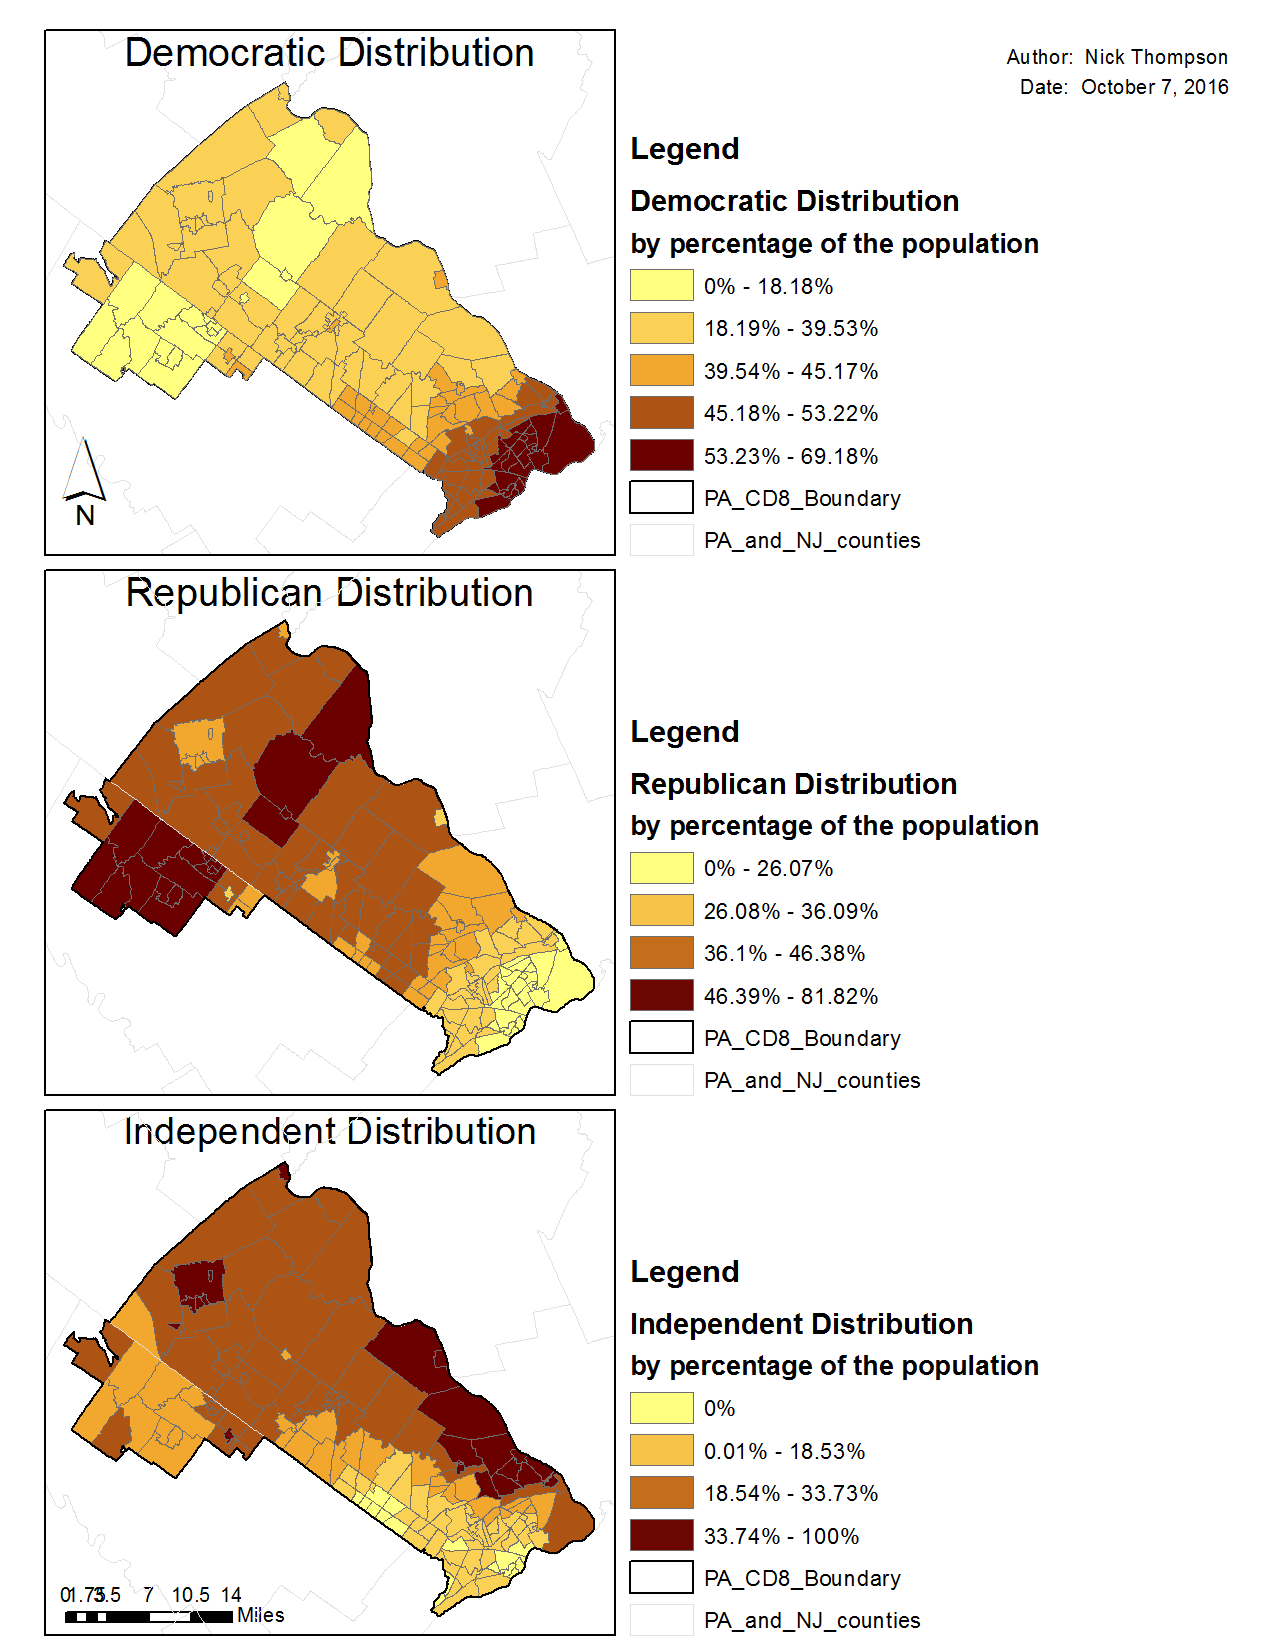
\includegraphics{question_2.png}
\caption{Figure 2: Parties in Space}
\end{figure}

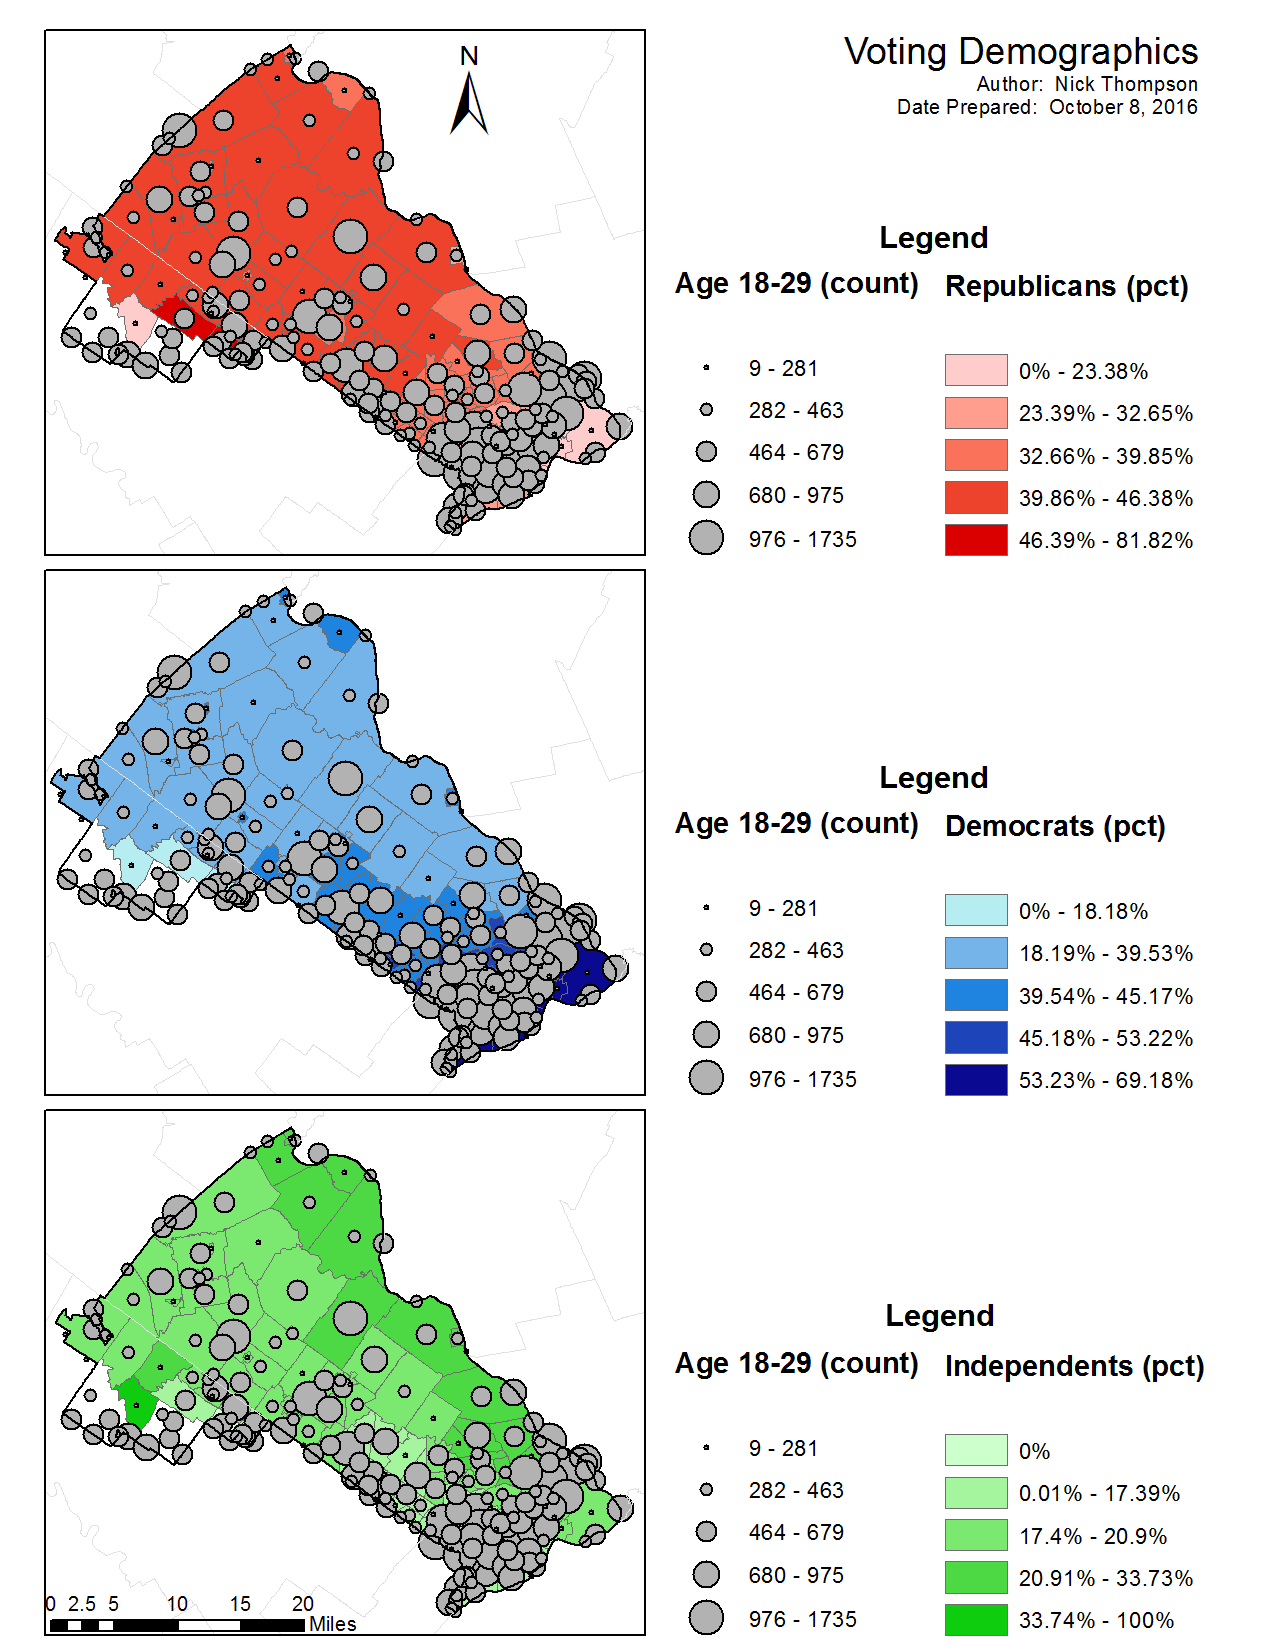
\includegraphics{question_3a.png} 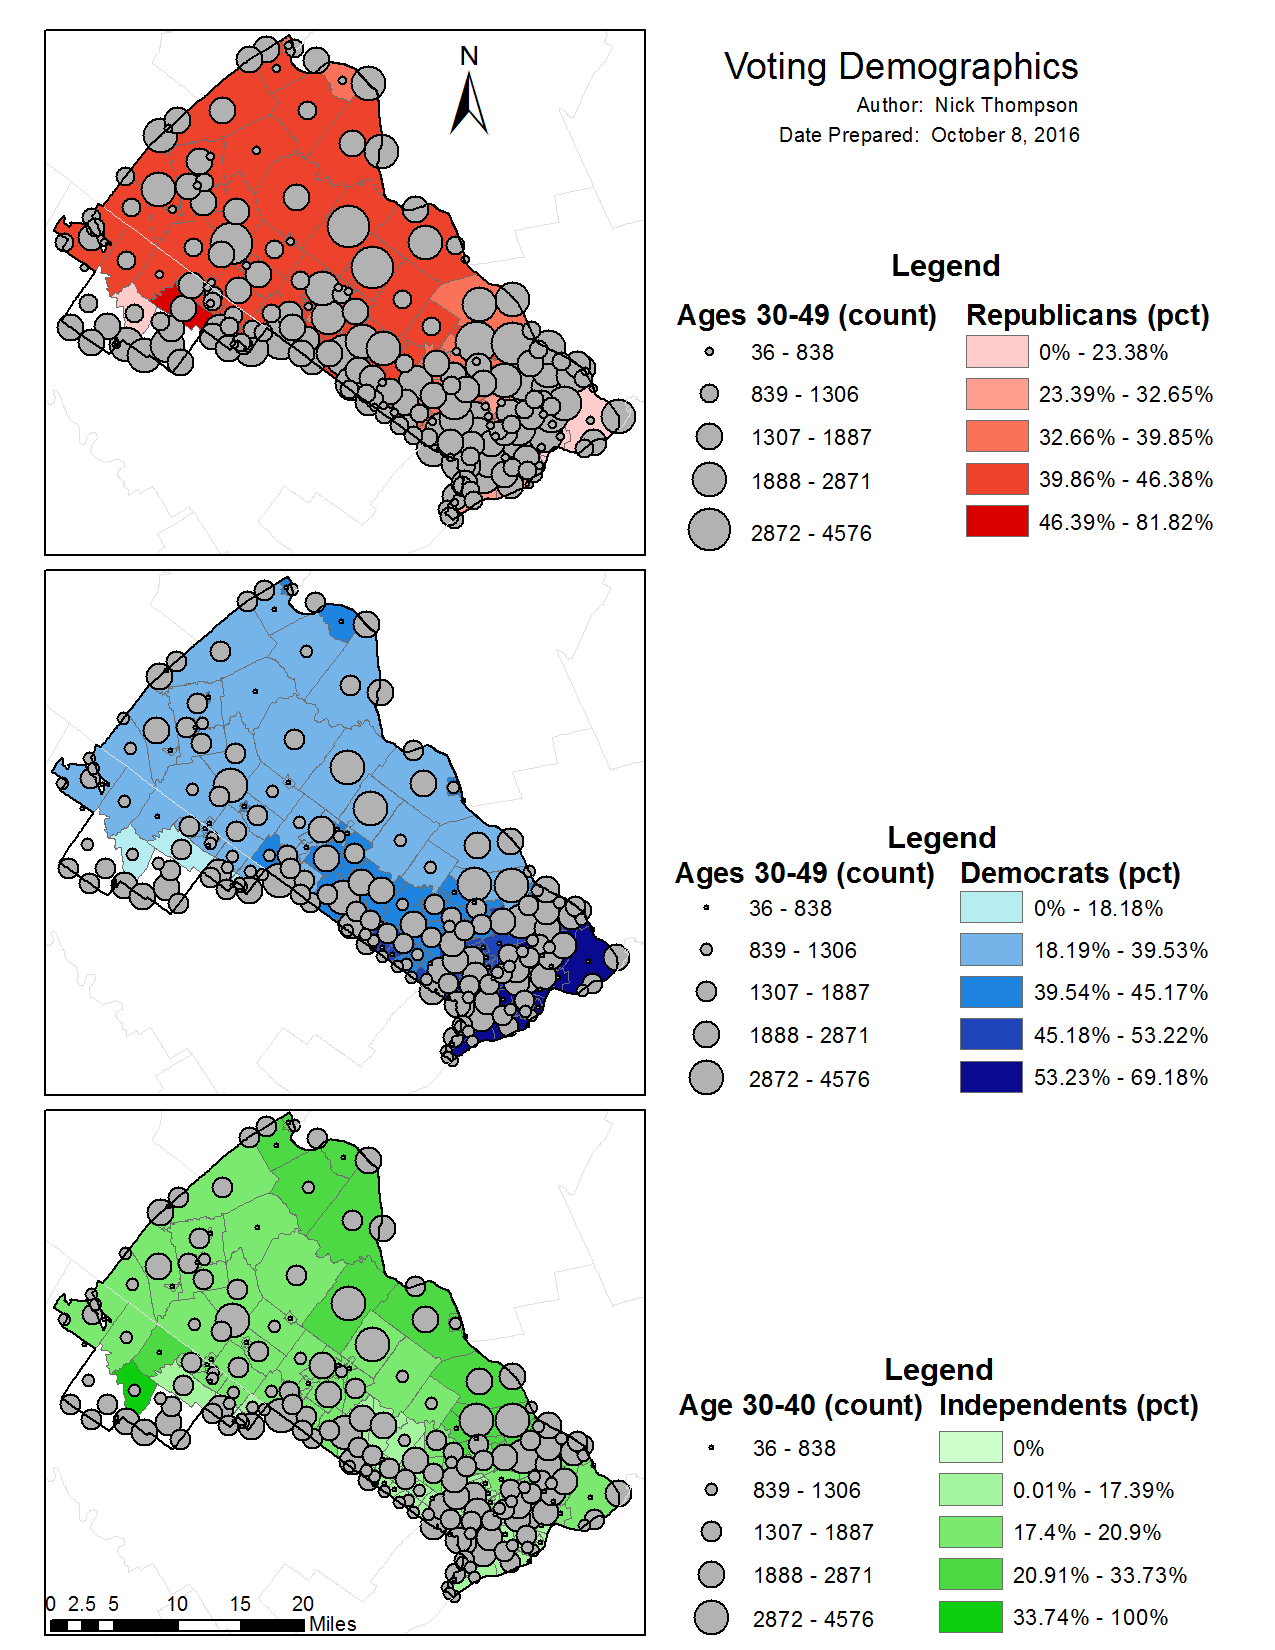
\includegraphics{question_3b.png}
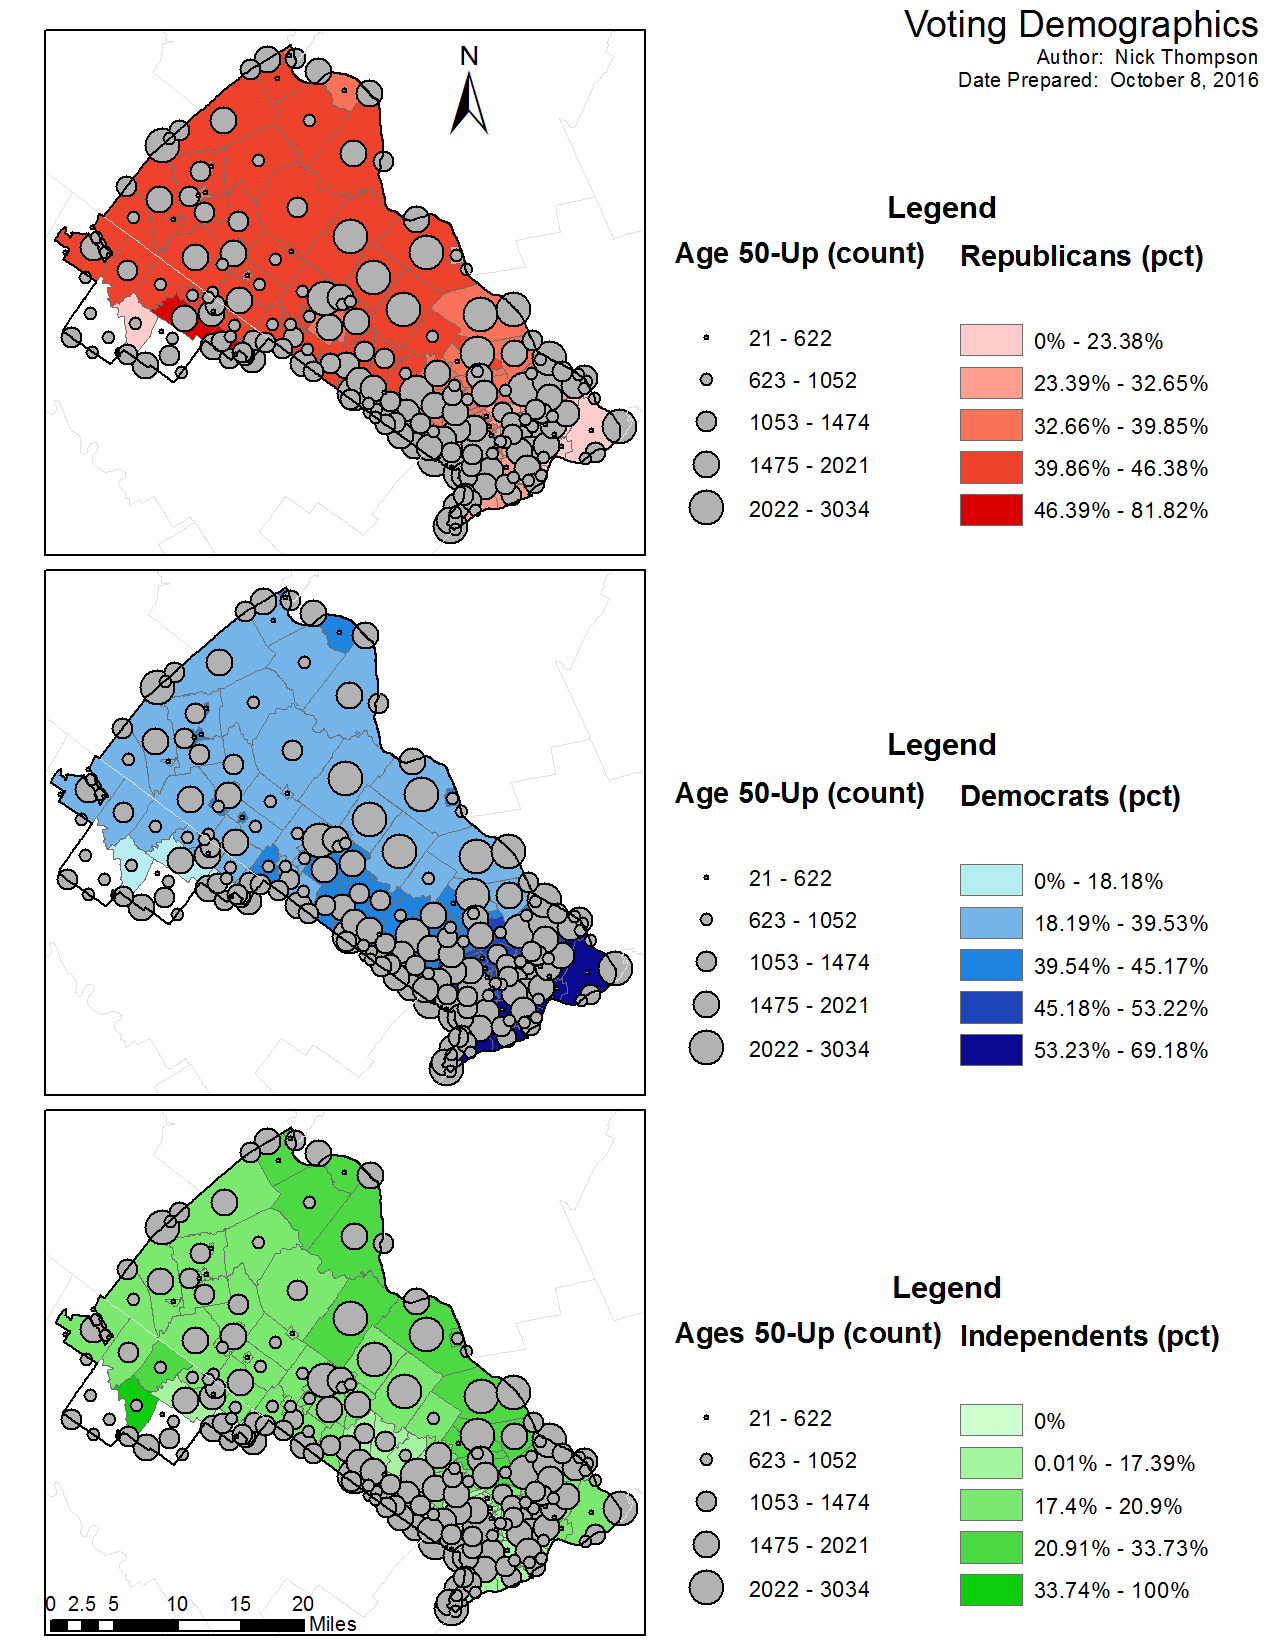
\includegraphics{question_3c.png}

\end{document}
